\chapter{AI Model for Detecting Depression}

\label{chap:ch4}

\section{Methodology}

\quad In order to develop an accurate AI model for detecting depression from textual data, the choice of the right model and the fine-tuning of its parameters are critical steps. In machine learning, selecting the most appropriate algorithm is very important to the success of any classifying task. This is also true in the case of depression detection, where the complexity and variability of the data demand an approach that is not only accurate but also can work on texts from different cultures. Looking at section 2.2, it was decided to use Random Forest (RF) as the AI model. 

In the context of this study focused on depression detection, the dataset resembles the Breast Cancer Wisconsin dataset (see Section 2.2), because the model is also a binary classifier. However, the model differentiates itself with a higher dimensionality, processing 119 input attributes for the English feature vector dataset and 86 for the Romanian one, which poses a greater complexity in feature representation and selection. For this dataset (Random Forest) RF achieved the highest accuracy at 97.85\%, suggesting it was the most successful in correctly identifying cases of breast cancer. It also had the highest kappa value of 95.03\%. Precision with RF was great as well, hitting a high of 98\%, while its recall was nearly as impressive at 97.9\%, showing its ability to identify most of the positive cases.

For processing the datasets LIWC-22 was used for the original dataset in English and LIWC-2015 for the Romanian translated dataset. This results in the feature vectors that contain numbers associated with each category presented in Figures \ref{LIWC22EnglishDicF1} and \ref{LIWC22EnglishDicF2} for the English 2022 dictionary (119 features), respectively Figures \ref{LIWC2015RomanianDicF1} and \ref{LIWC2015RomanianDicF2} for the Romanian 2015 dictionary (86 features). Except for "Word Count" which represents the number of words in the input text which is a whole number, all the numbers are rational. This comes from the fact that LIWC attributes to a word multiple categories, each with its specific score. Take the word "mad" — it's included in the anger dictionary. Consider "mad" usually shows some level of anger. But sometimes, it means joy ("he’s mad for her") or insanity ("mad as a hatter"). Thankfully, this rarely causes issues because LIWC uses probabilistic language models. If "mad" is used to show positive emotion in a sentence, the writer would typically use other positive words too and fewer anger words. This would give a high positive emotion score and a low anger score.

The resulted feature vectors are then used to train and evaluate the Random Forrest Classifier. There are 3 experiments detailed in the following section. The resulted models are saved and then used to classify the user input in the developed chrome extension. All steps of the proposed approach can be visualized in Figure \ref{proposedApproachFlow}.

\begin{figure}[htbp]
	\centering
		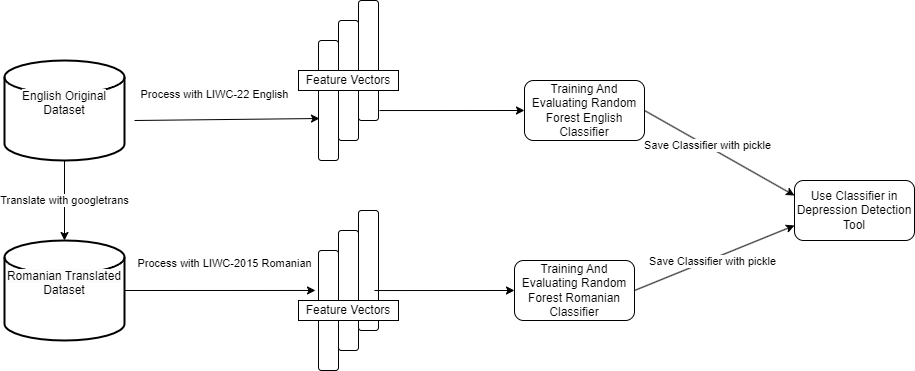
\includegraphics[scale=0.47]{LaTeX Bachelor Thesis Depression Signs Detection/figures/FlowModelWhite.png}
	\caption{Proposed Approach Flow}
	\label{proposedApproachFlow}
\end{figure}


\section{Experiments}

\quad To achieve an optimal model, it is essential to explore various training methodologies. This section describes the procedures followed in training the model. There are three experiments: two for the original dataset in English and one for the Romanian translated dataset. The classification flow for them can be visualized in Figure \ref{experimentsFlow}.

\begin{figure}[htbp]
	\centering
		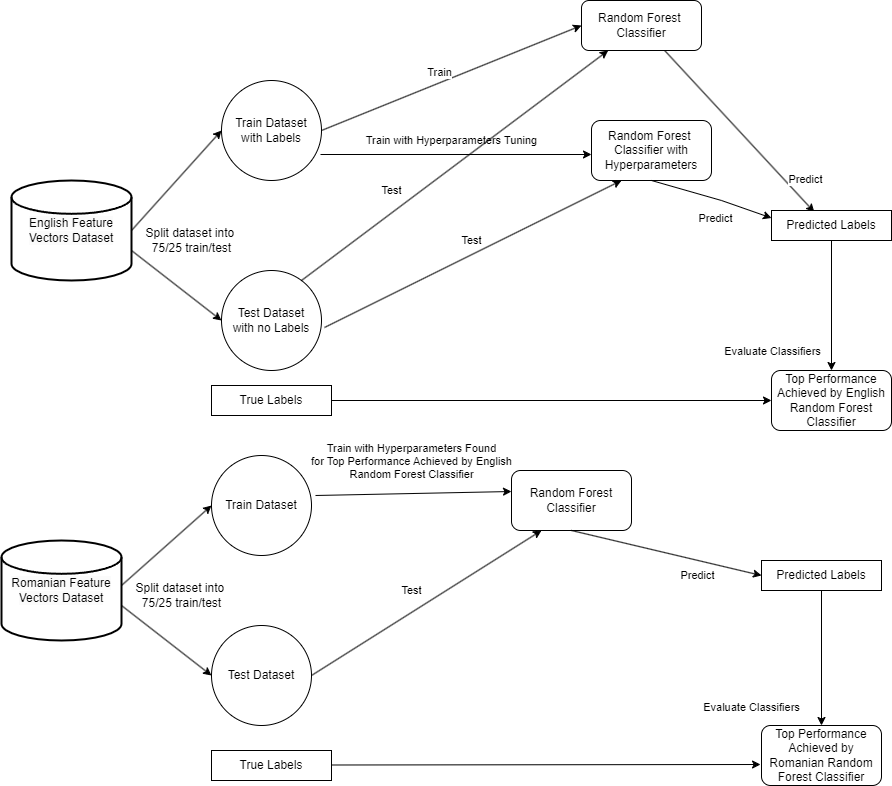
\includegraphics[scale=0.5]{LaTeX Bachelor Thesis Depression Signs Detection/figures/ClassificationFlowWhite.drawio (1).png}
	\caption{Experiments Flow}
	\label{experimentsFlow}
\end{figure}

\subsection{First Experiment for English Language}

\quad In the initial training experiment, all available features were utilized without any adjustments to hyperparameters. The default settings of the Random Forest Classifier from sklearn were applied \cite{sklearn_api}. The dataset was partitioned in a 75/25 train/test split, ensuring an equal distribution of positive and negative cases by using the stratify option, as illustrated in Figure \ref{codeTrainRF}.

\begin{figure}[htbp]
	\centering
		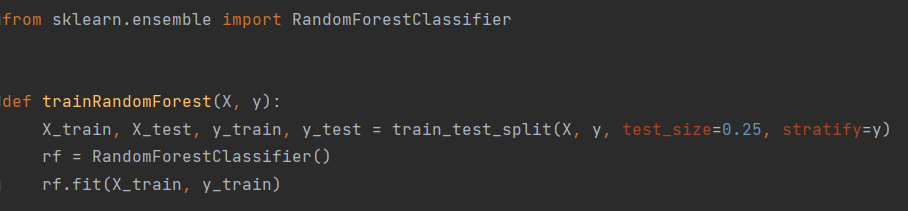
\includegraphics[scale=0.6]{LaTeX Bachelor Thesis Depression Signs Detection/figures/codeTrainingRF.png}
	\caption{Python code used for the initial training of the Random Forest Classifier}
	\label{codeTrainRF}
\end{figure}

The first experiment's results reveal a strong performance across the chosen metrics. The Classification Metrics plot shows high values for Accuracy (0.96), Precision (0.99), Recall (0.93), and F1 Score (0.96), indicating an efficient model with a balanced approach to both relevance (precision) and completeness (recall) \ref{classificationMetricsFirstExperiment}.

\begin{figure}[htbp]
	\centering
		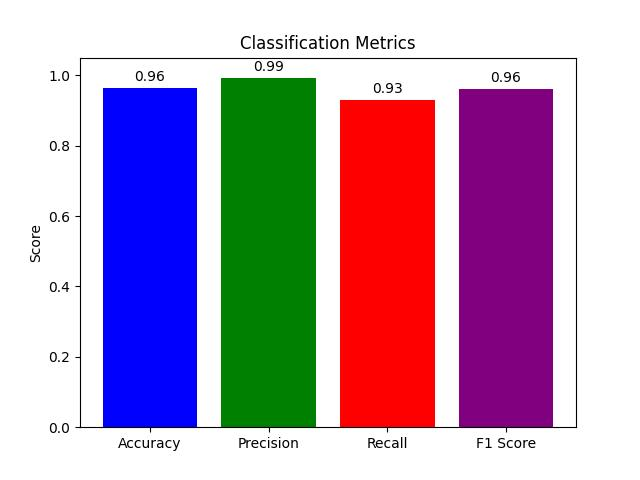
\includegraphics[scale=0.8]{LaTeX Bachelor Thesis Depression Signs Detection/figures/metrics/experiment1English/classificationMetrics.jpg}
	\caption{Classification Metrics - First Experiment}
	\label{classificationMetricsFirstExperiment}
\end{figure}

The Confusion Matrix provides a visual confirmation of the model's performance, with a high number of true positives (891) and true negatives (969), and relatively few false positives (6) and false negatives (67) \ref{confusionMatrixFirstExperiment}. This suggests the model has more problems when finding depression.

\begin{figure}[htbp]
	\centering
		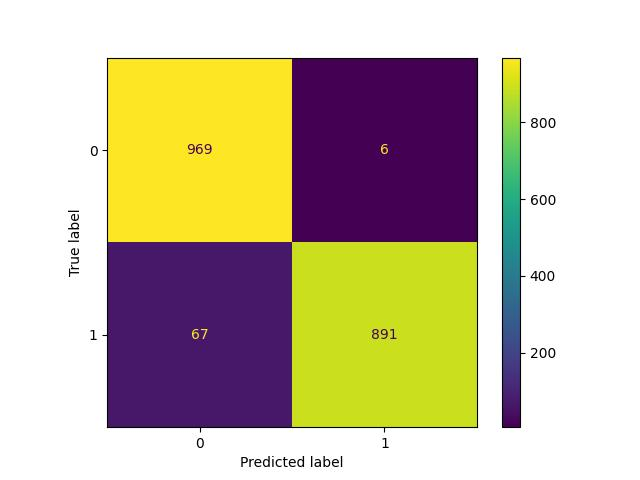
\includegraphics[scale=0.8]{LaTeX Bachelor Thesis Depression Signs Detection/figures/metrics/experiment1English/confusionMatrix.jpg}
	\caption{Confusion Matrix - First Experiment}
	\label{confusionMatrixFirstExperiment}
\end{figure}

% Looking at the ROC Curve, the model demonstrates an excellent ability to distinguish between the classes, as evidenced by the area under the curve (AUC) being close to 1 (0.99) \ref{rocCurveFirstExperiment}. This suggests that the model has a good discrimination capability with a high true positive rate and a low false positive rate across different thresholds.

% \begin{figure}[htbp]
% 	\centering
% 		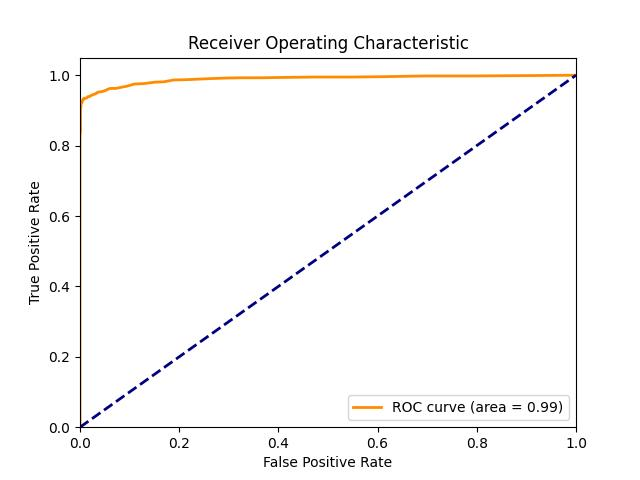
\includegraphics[scale=0.8]{LaTeX Bachelor Thesis Depression Signs Detection/figures/metrics/experiment1English/roc_curve.jpg}
% 	\caption{ROC Curve First Experiment}
% 	\label{rocCurveFirstExperiment}
% \end{figure}

The Top 10 Feature Importances plot indicates which features have the most influence on the model's predictions. The leading features, labeled as 'WC' (Word Count) and 'WPS' (Words per Sentence), seem to be the most significant drivers, with the others contributing to varying lesser degrees \ref{top10FeaturesFirstExperiment}. This shows us that the length of the given text is very important in order for the model to give an accurate prediction.

\begin{figure}[htbp]
	\centering
		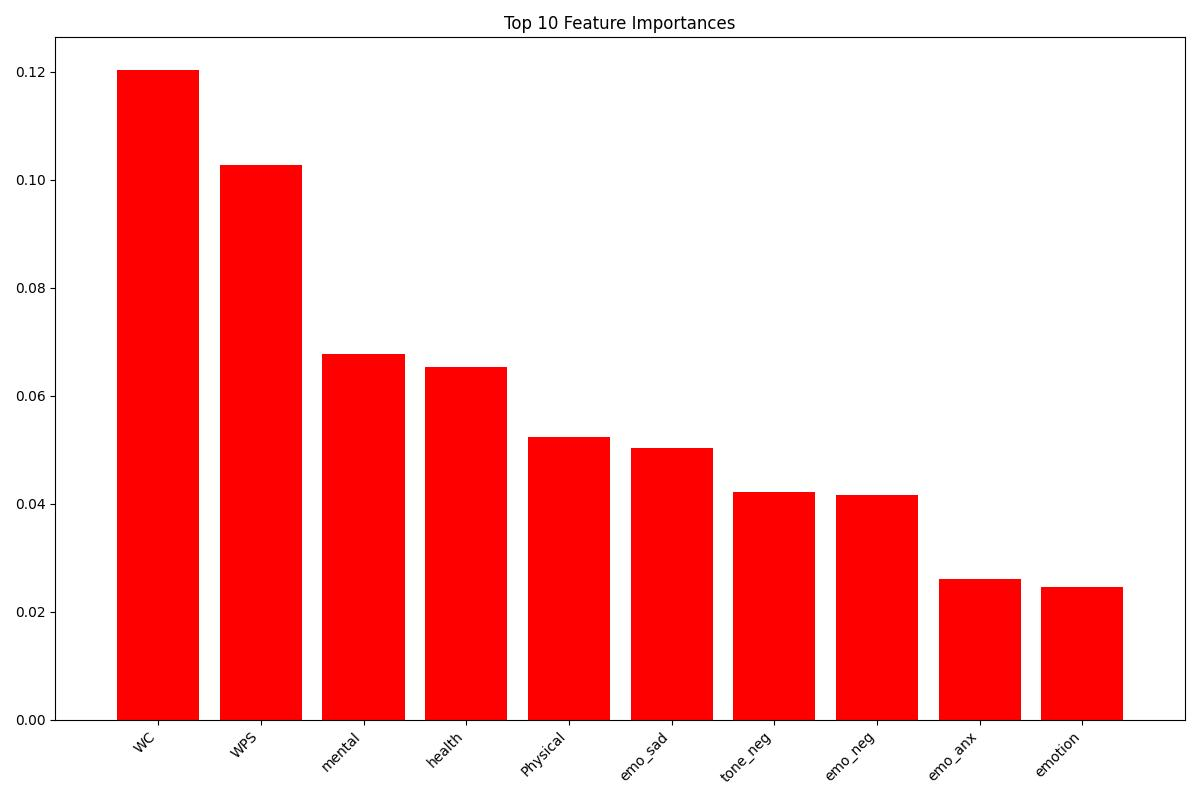
\includegraphics[scale=0.5]{LaTeX Bachelor Thesis Depression Signs Detection/figures/metrics/experiment1English/top10features.jpg}
	\caption{Top 10 Feature Importances -  First Experiment}
	\label{top10FeaturesFirstExperiment}
\end{figure}

Overall, the model appears to be highly effective, with strong performance indicators, which seems to be the result of the analysis done for choosing the pre-processing methods and classifier, namely LIWC \cite{boyd2022development} and Random Forrest.

\subsection{Second Experiment for English Language}
The selection of Random Forest hyperparameters is guided by the study \cite{probst2019hyperparameters}. The adjusted hyperparameters are:

\begin{itemize}
  \item \textbf{mtry}: This represents the number of features considered for splitting at each node. Lower values promote tree diversity and are beneficial when there are many relevant predictors. Given the large feature set, a value lower than the default square root of the number of features is suggested to prevent dominant features from overshadowing others.
  \item \textbf{Number of Trees}: A sufficient number of trees ensures stable predictions and importance estimates. While more trees generally improve model performance, beyond a certain point the marginal gains diminish. For practical purposes, between 500 to 1000 trees are recommended.
  \item \textbf{Node Size}: The node size controls the depth of the tree. Smaller node sizes can potentially lead to over-fitting, particularly when the number of features is high. A larger than 1 node size is preferred to mitigate this risk and improve computational efficiency.
  \item \textbf{Sample Size}: The proportion of data used for training each tree. Smaller sample sizes lead to more diversity but can decrease individual tree accuracy. Optimal sample size needs to be problem-specific but sampling a subset, such as between 20\% and 90\% of the data, can yield good results while reducing runtime. 
\end{itemize}

These hyperparameters were tuned using Sequential Model-Based Optimization (SMBO) to determine their optimal values while considering the Area Under the ROC Curve (AUC) as the performance metric \cite{probst2019hyperparameters}.

For the depression binary classifier multiple configurations were tested. It was noticed that the optimal ranges for the hyperparameters were:
\begin{itemize}
    \item \textbf{mtry}: between 6 and 10
    \item \textbf{Number of trees}: between 700 and 1000
    \item \textbf{Node Size}: between 3 and 9
    \item \textbf{Sample size}: between 6 and 9
\end{itemize}

After training with all combinations of the mentioned ranges, the one who got the best results was 6 for mtry, 900 for number of trees, 3 for node size and 8 for sample size. The same metrics as in the first experiment were used to analyze the performance of the model and improvements were seen. For the classification metrics accuracy(0.97) has improved by 0.01, precision stayed the same, recall(0.96) was the one who improved the most by 0.03, and F1-score(0.97) improved by 0.01. These values can be seen comparing Figure \ref{classificationMetricsFirstExperiment}, which shows the classification metrics for the first experiment, with Figure \ref{classificationMetricsSecondExperiment}, which shows them for the second experiment. This shows that because of hyperparameters tuning, it succeeded in improving the part where the model from the first experiment lacked.

\begin{figure}[htbp]
	\centering
		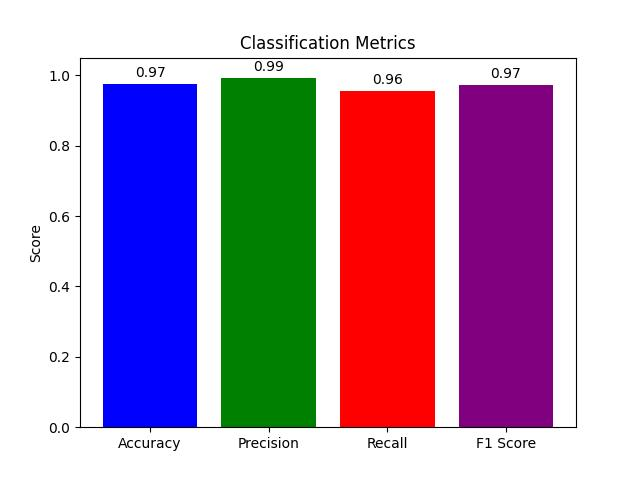
\includegraphics[scale=0.8]{LaTeX Bachelor Thesis Depression Signs Detection/figures/metrics/experiment2English/classificationMetrics.jpg}
	\caption{Classification Metrics - Second Experiment}
	\label{classificationMetricsSecondExperiment}
\end{figure}

In the case of the confusion matrix for the second experiment \ref{confusionMatriSecondExperiment} it can be discovered that in comparison with the one for the first experiment \ref{confusionMatrixFirstExperiment}, as can the improvement of recall also tell, the values of the false positives decreased, from 67 to 43.

\begin{figure}[htbp]
	\centering
		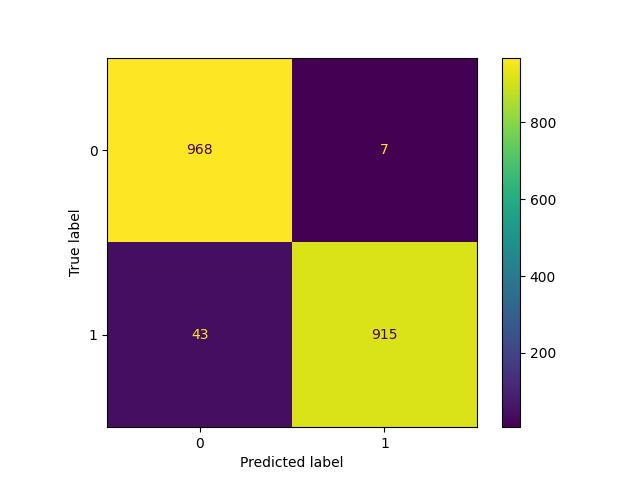
\includegraphics[scale=0.8]{LaTeX Bachelor Thesis Depression Signs Detection/figures/metrics/experiment2English/confusionMatrix.jpg}
	\caption{Confusion Matrix - Second Experiment}
	\label{confusionMatriSecondExperiment}
\end{figure}

% For the ROC curve for this experiment \ref{rocCurveSecondExperiment}, the area stayed the same when looking to the first two digits, but an improvement of the true positive rate can be noticed from the initial experiment \ref{rocCurveFirstExperiment}.

% \begin{figure}[htbp]
% 	\centering
% 		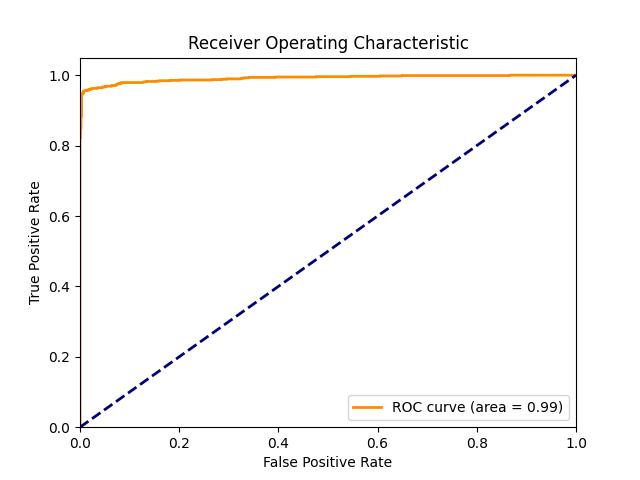
\includegraphics[scale=0.8]{LaTeX Bachelor Thesis Depression Signs Detection/figures/metrics/experiment2English/roc_curve.jpg}
% 	\caption{ROC Curve Second Experiment}
% 	\label{rocCurveSecondExperiment}
% \end{figure}

Seeing the top 10 features of the second experiment \ref{top10FeaturesSecondExperiment}, it was noticed that in comparison with the initial one \ref{top10FeaturesFirstExperiment} that even though WC (Word Count) and WS (Words per Sentence) are the still the most important features, they are now by much less, from 0.12 and 0.10 to both being at 0.09. This shows that now there are more features taken into account when the model makes the classification and each is more influential. Also it is remarked that a feature in the first ten was changed, namely emo\_anx (anxiety) with cause (causation).

\begin{figure}[htbp]
	\centering
		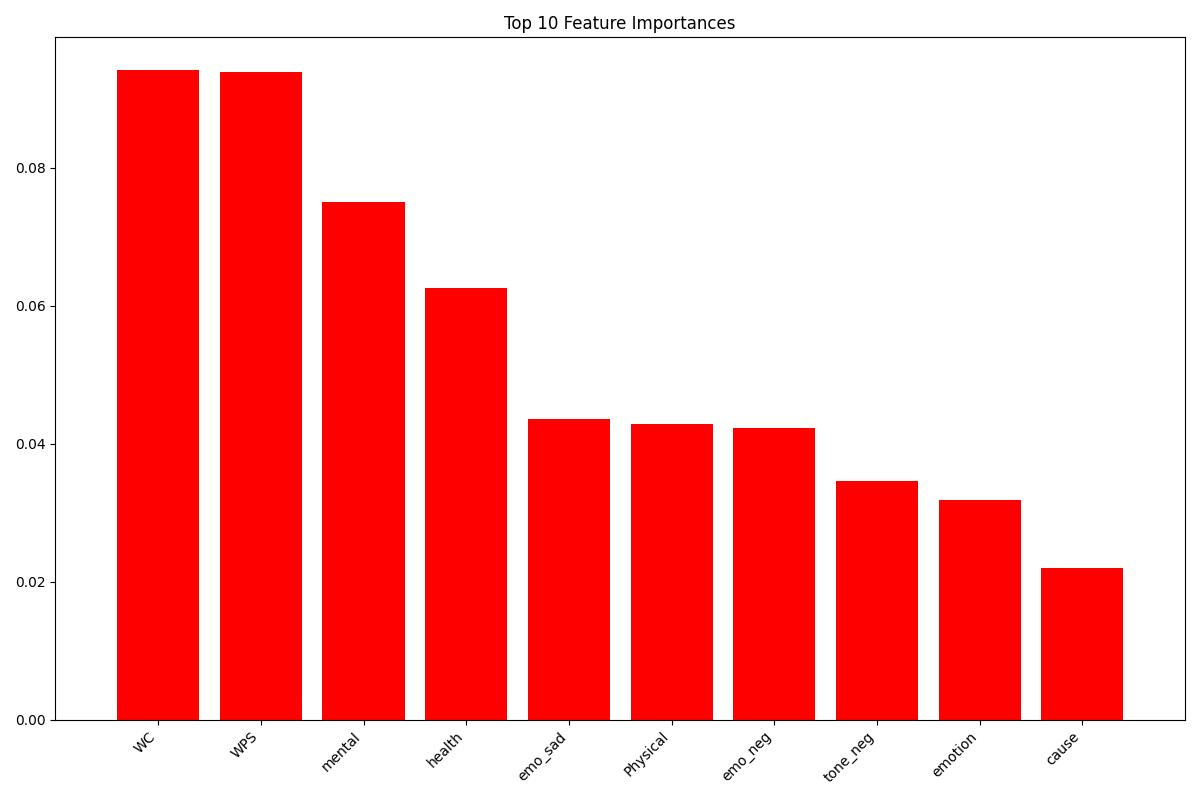
\includegraphics[scale=0.5]{LaTeX Bachelor Thesis Depression Signs Detection/figures/metrics/experiment2English/top10features.jpg}
	\caption{Top 10 Feature Importances - Second Experiment}
	\label{top10FeaturesSecondExperiment}
\end{figure}

\subsection{Experiment for Romanian Language}

\quad For the Romanian language model, the methodology was replicated consistently. LIWC served as the tool for preprocessing the data. However, the most recent English dictionary for LIWC-22 has not been translated into Romanian. The latest available version for Romanian is the LIWC-2015 dictionary, which contains only 86 features, compared to the 119 features available in the English version.

The training approach was aligned with the methodology used for the English model during the second experiment. The hyperparameters and the proportion of training to testing data remain consistent:

\begin{itemize}
\item \textbf{train/test split}: Maintained at 75/25, using stratification based on the 'is\_depression' label
\item \textbf{mtry}: 6
\item \textbf{Number of trees}: 900
\item \textbf{Node Size}: 3
\item \textbf{Sample size}: 8
\end{itemize}

This methodology facilitates a direct comparison between the performance of the Romanian and English models, ensuring consistent evaluation criteria across both. The same metrics were used for analysis. In terms of classification metrics, the most notable discrepancy arises in recall, where the Romanian model scores 0.87, falling short of the English model's 0.96 by 9 percentage points. Additionally, both accuracy and the F1-score have diminished by 0.05, while precision experienced the least impact, decreasing from 0.99 to 0.97. These metrics are illustrated in Figure \ref{classificationMetricsSecondExperiment} for the English model and in Figure \ref{classificationMetricsRomanianExperiment} for the Romanian model.

The diminished recall in the Romanian model suggests it is less adept at identifying true positive cases as compared to the English model. This lower performance may come from the nuances lost during the translation of the dataset from English to Romanian using the Googletrans library \cite{googletranslib}. Such translation challenges could contribute to the model’s reduced effectiveness, highlighting the influence of linguistic or cultural differences on the model’s ability to generalize across languages. The smaller reductions in accuracy and F1-score indicate that while the model is somewhat less effective overall, it still maintains a reasonable level of precision.

\begin{figure}[htbp]
	\centering
		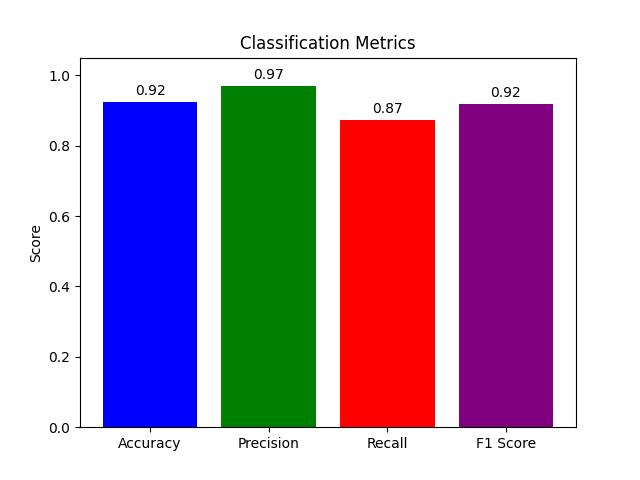
\includegraphics[scale=0.8]{LaTeX Bachelor Thesis Depression Signs Detection/figures/metrics/experimentRomanian/classificationMetrics.jpg}
	\caption{Classification Metrics - Romanian Model}
	\label{classificationMetricsRomanianExperiment}
\end{figure}

The confusion matrix \ref{confusionMatrixRomanianExperiment} illustrates a significant increase in false positives, rising from 43 in the English model \ref{confusionMatriSecondExperiment} to 123 in the Romanian model. However, the rise in false negatives was less marked, increasing from 7 to 26.

\begin{figure}[htbp]
	\centering
		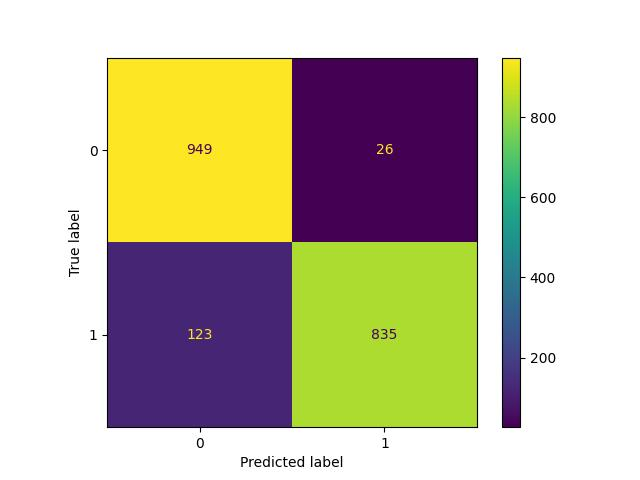
\includegraphics[scale=0.8]{LaTeX Bachelor Thesis Depression Signs Detection/figures/metrics/experimentRomanian/confusionMatrix.jpg}
	\caption{Confusion Matrix - Romanian Model}
	\label{confusionMatrixRomanianExperiment}
\end{figure}

% Regarding the ROC curve, the Area Under the Curve (AUC) experienced a slight decrease of 0.01, as depicted in Figure \ref{rocCurveRomanianExperiment} compared to Figure \ref{rocCurveSecondExperiment}. These metrics collectively indicate that the issues observed during the experimentation with the English model are more pronounced in the Romanian classifier.

% \begin{figure}[htbp]
% 	\centering
% 		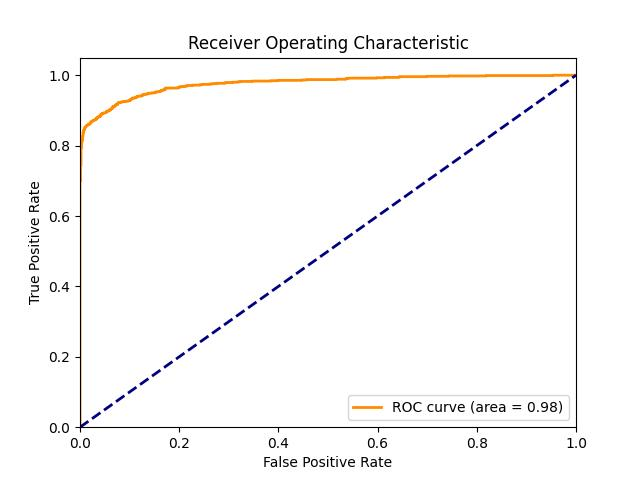
\includegraphics[scale=0.8]{LaTeX Bachelor Thesis Depression Signs Detection/figures/metrics/experimentRomanian/roc_curve.jpg}
% 	\caption{ROC Curve Romanian Model}
% 	\label{rocCurveRomanianExperiment}
% \end{figure}

The most significant features for the Romanian classifier \ref{top10FeaturesRomanianExperiment} align more closely with those observed in the initial experiment for the English model \ref{top10FeaturesFirstExperiment}. Notably, Word Count (WC) has risen above 0.12, surpassing the importance it held in the first experiment. This contrasts with the improvements seen in the second English experiment \ref{top10FeaturesSecondExperiment}, where a diminished reliance on WC and WPS (Words per Sentence) indicated a broader array of features influencing the English classifier’s decisions. However, this diversification does not appear to extend to the Romanian model.

Some features remain consistent with the English LIWC-22 dictionary features listed in the top 10 for the second experiment; for instance, "sad" aligns with "emo\_sad", and both "cause" and "health" are both present and "negemo" is the same as "emo\_neg". The "anx" feature mirrors "emo\_anx" from the first experiment’s top features. The presence of "Period" suggests that the Googletrans library has introduced punctuation marks, which have become a significant element. The evolution from LIWC-2015 to LIWC-22 is further evidenced by the removal of the "interrog" category in the Romanian model’s top 10 features, which was dropped in LIWC-22 due to its low base rates, internal reliability, or infrequent usage, as noted in \cite{boyd2022development}. The "ipron" feature might also result from the machine translation process.

\begin{figure}[htbp]
	\centering
		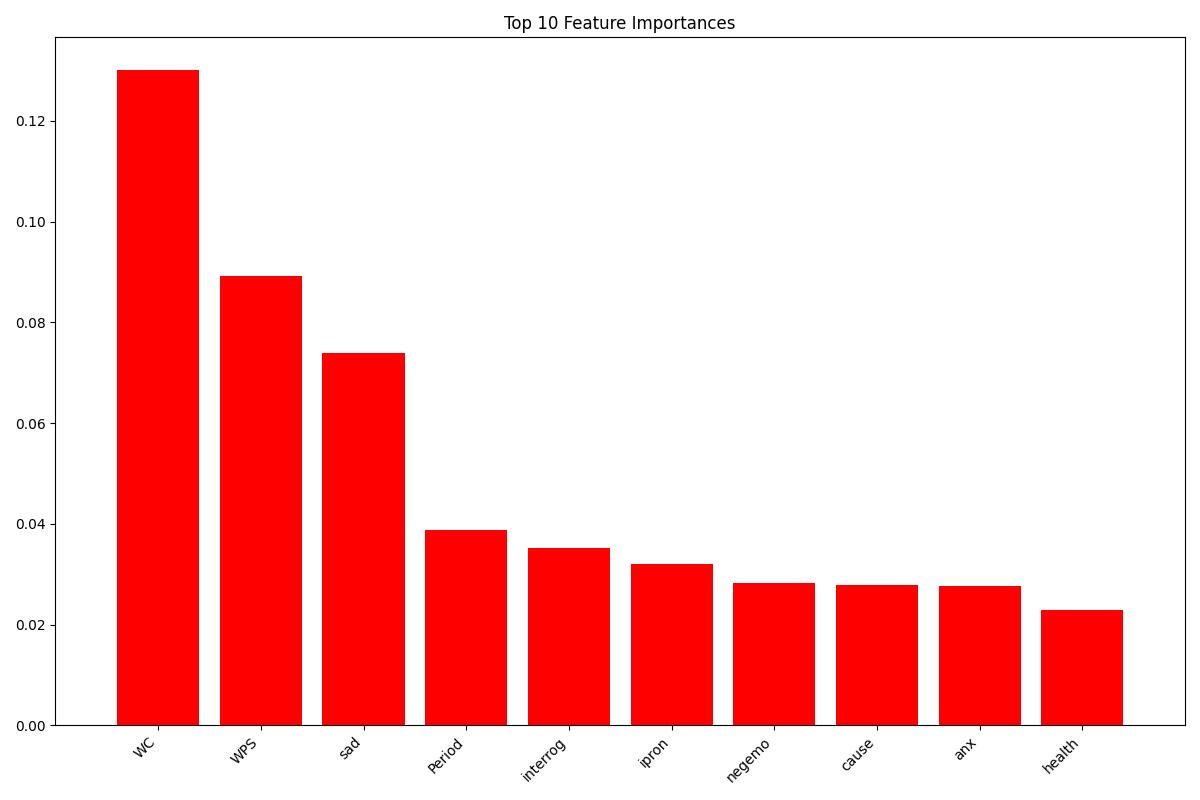
\includegraphics[scale=0.5]{LaTeX Bachelor Thesis Depression Signs Detection/figures/metrics/experimentRomanian/top10features.jpg}
	\caption{Top 10 Features - Romanian Model}
	\label{top10FeaturesRomanianExperiment}
\end{figure}

By looking at some examples from the dataset, we can see the differences between the two models more clearly.

\textbf{Example 1}: Both texts, English and the Romanian translation, are predicted by the models as depression, matching the dataset's label.
\begin{itemize}
    \item 
\textbf{English text}: "anyone else instead of sleeping more when depressed stay up all night to avoid the next day from coming sooner may be the social anxiety in me but life is so much more peaceful when everyone else is asleep and not expecting thing of you" 
\item
\textbf{Translated in Romanian}: "oricine altcineva în loc să doarmă mai mult atunci când este deprimat să stea treaz toată noaptea pentru a evita ca ziua următoare să vină mai devreme poate fi anxietatea socială din mine dar viața este mult mai liniștită când toți ceilalți doarme și nu așteaptă nimic de la tine" 
\end{itemize}

\textbf{Example 2}: The true label is depression and the English model predicts this correctly, but the Romanian one does not.

\begin{itemize}
    \item \textbf{English text}: "it s so pointless for me to still be alive my life is worthless why am i still here" 
    
    \item \textbf{Translated in Romanian} "este atât de inutil să fiu încă în viață viața mea este inutilă de ce sunt încă aici" are labeled as depression. 

\end{itemize}

\textbf{Example 3}: The text does not show depression, but  both models predict the input incorrectly.

\begin{itemize}
    \item \textbf{English text}: "i m starting to lose hope i feel like i m on auto pilot i m not living i m existing" 
    
    \item \textbf{Translated in Romanian}: "Încep să-mi pierd speranța simt că sunt pe pilot automat nu trăiesc exist"
\end{itemize}

This shows they might be too quick to call certain feelings depressive and while both models sometimes agree, they can also differ, especially with translations. The Romanian model needs more work, and both models tend to over-predict depression.






.


